%%%%%%%%%%%%%%%%%%%%%%%%%%%%%%%%%%%%%%%%%%%%%%%%%%%%%%%%%%%%%%%%%%%%%%%%
% RevTeX 4.1 LaTeX
% Kevin C. Young
% Scalable & Secure Systems Research (08961)
% Thu Mar  5 15:29:19 PST 2015
%%%%%%%%%%%%%%%%%%%%%%%%%%%%%%%%%%%%%%%%%%%%%%%%%%%%%%%%%%%%%%%%%%%%%%%%

\documentclass[aps,nofootinbib,pra,notitlepage,twocolumn]{revtex4-1}
\usepackage{amsfonts,amsmath,amssymb,amsthm}
 \usepackage{array,bm,color}
\usepackage{epsfig,graphicx,nomencl,revsymb4-1,upgreek,url}
\usepackage{hyperref}
\usepackage{algorithm}
\usepackage{algpseudocode}
\usepackage{graphicx}
\usepackage{calc}
\usepackage{tabularx}
\newcolumntype{Y}{>{\centering\arraybackslash}X}
\graphicspath{{./figures/}}
\hypersetup{colorlinks=true, pdfauthor=Anthony M. Polloreno, pdftitle=Robustly decorrelating errors with mixed quantum gates, citecolor=blue, linkcolor=blue}
\newcommand{\tr}{{\rm Tr\thinspace}}
\newcommand{\bra}[1]{\ensuremath{\left\langle{#1}\right\vert}}
\newcommand{\ket}[1]{\ensuremath{\left\vert{#1}\right\rangle}}
\newcommand{\braket}[2]{\left\langle #1 | #2 \right\rangle}
\newcommand{\ketbra}[2]{\left| #1 \right\rangle\!\!\!\,\left\langle #2 \right|}
\newcommand{\abs}[1]{\left\vert #1 \right\vert}
\newcommand{\expect}[1]{\ensuremath{\left\langle{#1}\right\rangle}}
\newcommand{\timeorder}{\ensuremath{\underset{\leftarrow}{\mathcal{T}}}}
\newcommand{\ident}{{\mathbb1}}
\newcommand{\order}[1]{\mathcal{O}\left( #1 \right)}
\newcommand{\diag}[1]{\mathrm{diag}\{#1\}}
\newcommand{\trans}[1]{#1^\mathsf{T}}
\newcommand{\T}{\mathsf{T}}
\newcommand{\erf}[1]{Eq.~(\ref{#1})}
\newcommand{\needcite}{{\color{blue}\textsuperscript{[citation needed]}}}
% \newcommand{\note}[1]{{\color{red}[#1]}}
\newcommand{\note}[1]{}
\newcommand{\kcy}[1]{{\color{red}[#1]\textsubscript{\rm{KCY}}}}
\newcommand{\amp}[1]{{\color{red}[#1]\textsubscript{\rm{AMP}}}}
\newcommand{\deriv}[0]{{\frac{d}{d\vec{\delta}}}}

\newcommand{\actual}{\ensuremath{\tilde{\mathsf{G}}}}
\newcommand{\target}{\ensuremath{{\mathsf{G}}}}
\newcommand{\error}{\ensuremath{{\mathsf{E}}}}
\newcommand{\generator}{\ensuremath{{\mathsf{G}}}}
\newcommand{\vectorize}[1]{\ensuremath{\mathsf{vec}\left(#1\right)}}
\def\id{\mbox{\small 1} \!\! \mbox{1}}

%-------------Header begins here----------------------------------------
\begin{document}
\title{Robustly decorrelating errors with mixed quantum gates}

\author{Anthony M. Polloreno}
\email[Email: ]{ampolloreno@gmail.com}
\affiliation{Rigetti Computing, Berkeley, CA}

\author{Kevin C. Young}
\affiliation{Quantum Performance Laboratory, Sandia National Laboratories, Livermore, CA}

\date{\today}

\begin{abstract}
\noindent Coherent errors in quantum operations are ubiquitous. Whether arising from spurious environmental couplings or errors in control fields, such errors can accumulate rapidly and degrade the performance of a quantum circuit significantly more than an average gate fidelity may indicate. As Hastings \cite{Hastings2017} and Campbell \cite{Campbell2017} have recently shown, by replacing the deterministic implementation of a quantum gate with a randomized ensemble of implementations, on can dramatically suppress coherent errors. Our work begins by reformulating the results of Hastings and Campbell as a quantum optimal control problem. We then discuss a family of convex programs designed to improve the performance, implementability, and robustness of the resulting mixed quantum gates. Finally, we implement these mixed quantum gates on a superconducting qubit and discuss randomized benchmarking results consistent with a marked reduction in the coherent error.\\
{[1]} M. B. Hastings, \emph{Quantum Information \& Computation} 17, 488 (2017). \\
{[2]} E. Campbell, \emph{Physical Review A} 95, 042306 (2017).
\end{abstract}

\pacs{}

\maketitle


% ==============================================================================
% Section: Introduction
% ==============================================================================
\section{Introduction}
\label{sec:introduction}
\noindent The ultimate impact of a gate error on a quantum circuit depends strongly on both the magnitude and the nature of the error. Systematic, or \emph{coherent}, errors can arise from poorly calibrated controls or approximate gate compilations that induce repeatable, undesired unitary errors on the state of a quantum information processor (QIP). Errors of this type are correlated in time may add up constructively or destructively, depending on the circuit. They are are  computationally expensive to model and, because coherent errors may amplify when gates are repeated, it can be difficult to place tight analytic bounds on circuit performance \cite{Beale2018}. Contrast this against random, or \emph{stochastic}, errors which often result from high-frequency noise in the controls or the environment. Systems with stochastic errors can usually be accurately modeled by defining a rate of various discrete errors in the system, such as a bit flips or phase flips. These errors are significantly easier to simulate on a classical computer, and their impact on quantum circuits is much easier to estimate \cite{Beale2018}.

\begin{figure}[t]
  \centering
  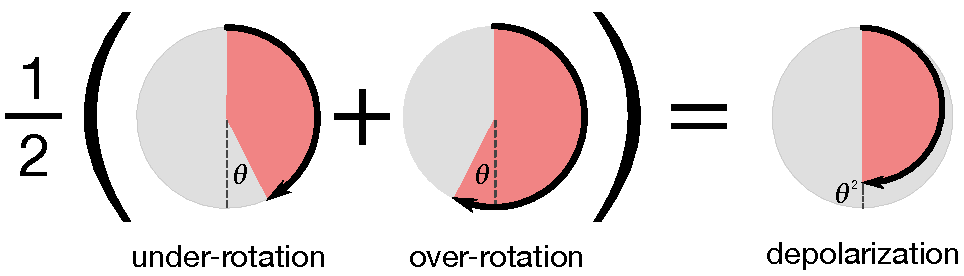
\includegraphics[width=\columnwidth]{simple_example.pdf}
  \caption{An example of a mixed quantum gate. Using optimal control, two implementations of a $Z_\pi$ gate are designed to have equal and opposite sensitivity to errors (if one implementation over-rotates by angle $\theta$, then the other \emph{under}-rotates by $\theta$). Each time the gate is used, one of these implementations is chosen at random. The resulting quantum channel is equivalent to a perfect implementation of the gate followed by dephasing of $\order{\theta^2}$.}
  \label{fig:simple_example}
\end{figure}

Recent works by Campbell \cite{Campbell2017,1811.08017} and Hastings \cite{Hastings2017} have shown that coherent noise can be strongly suppressed by probabilistically mixing several distinct implementations of the target quantum gates. They focus on errors arising from various gate compilations, such as the Solovey-Kitaev algorithm, for which any lingering approximation errors are generally coherent, even if the native gates are perfect. Different approximate gate compilations of the same target unitary will almost certainly result in a different unitary error. So by selecting from these various compilations at random, the resulting quantum channel becomes a mixture of unitaries \cite{DBLP:journals/corr/cs-CC-0012017}, which can have significantly less coherent error than any single compilation on its own. A very simple example of this reduction in coherent error by mixed quantum gates is illustrated in Fig.~\ref{fig:simple_example}. 

In this article, we extend the work of Campbell and Hastings to numerically optimized quantum gates, and show that the advantages of this approach can be made robust to drift in the gate implementations. We demonstrate that, depending on what properties of the resulting channel are desired, different numerical optimization targets may be preferred. We present an experimental implementation of single-qubit mixed unitary controls on a superconducting qubit testbed at Rigetti Computing. Using randomized benchmarking, we are able to show a marked improvement in error rates, as well as a reduced variance in circuit outcome probabilities, consistent with a reduction in the coherence of the error \cite{Ball2016}. We further apply our methods in simulation where we construct single- and two-qubit mixed unitary controls which are robust to drift and uncertainty in the control parameters.

% Reducing the coherence of a the quantum gate error 

% 
% 

% It has long been recognized, however, that one may inject additional decorrelating randomness 

% By injecting additional decorrelating randomness into the system,  

% By introducing additional decorrelating randomness, a number of techniques are able to convert coherent  errors into stochastic errors. 

% By introducing intentional additional randomness to the 
% The gate-to-gate correlations that occur in the presence of coherent noise 

% \note{don't define diamond norm here}
% The diamond distance can be used to bound the total variation distance (TVD) of a quantum circuit, but it is in general sensitive at first order to repeated application of a gate with coherent errors. For long circuits, this can add up extremely quickly, and while these errors can often be identified and reconstructed using various tomographic techniques, their impact on a given quantum  difficult to predict. Additionally, despite the relative ease of modeling stochastic errors, coherent errors are often much more likely to appear in QIPs. 




%Drifting control parameters or environmental variables can easily have long correlation times that result in errors which are strongly coherent over the length of a quantum circuit. 


% ==============================================================================
% Section: Mathematical preliminaries
% ==============================================================================
\section{Representing Errors }
\label{sec:representing_quantum_gates}

\subsection{Representing Errors in Quantum Gates}
\noindent Suppose that one wishes to apply a unitary gate, $\mathsf{G}$, on some quantum device. Implementing this operation on a real system generally involves the application of a sequence of classical control fields to some set of qubits.  But fluctuations in the environment or imperfections in these controls can cause the state of the qubits to change in a way that is different from what was intended, \emph{i.e.}, there are errors in the gate. If the device is fairly stable with time and context\cite{Rudinger2019}, then we can accurately model the gate action using a completely positive, trace-preserving (CPTP) map, $\mathsf{\tilde G}$ acting on the Hilbert space of the target qubits. This map can always be written as $\mathsf{\tilde G} = \mathsf{E}\circ\mathsf{G}$, where $\mathsf{E} = \mathsf{\tilde G}\circ\mathsf{G}^{-1}$ is the \emph{error map}, which is itself CPTP because $\mathsf{G}$ is unitary.

CPTP maps possess a number of useful representations, including Kraus operators\cite{1983}, Choi matrices\cite{Choi1975}, and Jamiolkowsi states\cite{yczkowski2004}. But for the purposes of this article, the \emph{process matrix} representation will be particularly convenient\cite{OBrien2004}, and we shall denote the process matrix associated with a given CPTP map $\mathsf{G}$ with the corresponding calligraphic character, $\mathcal{G}$. For a $d$-dimensional quantum state, the process matrix is a $d^2\times d^2$ matrix. A key feature of process matrices is that they are composable and act through the usual matrix multiplication on the vectorized quantum state:
\begin{align}
	\vectorize{\mathsf{\tilde G}(\rho)}
		&= \mathcal{\tilde G}\cdot\vectorize{\rho} \\
		&= \mathcal{E}\cdot\mathcal{G}\cdot\vectorize{\rho}
\end{align}
We shall work in the basis of Pauli matrices, defining $\Sigma = \left\{I, \sigma_x, \sigma_y, \sigma_z\right\}^{\otimes n}$ as the collection of all $4^n$ $n$-qubit Pauli operators (including the identity).  In this basis,
\begin{equation}
  \vectorize{\rho}_i = \tr\!\left(\rho \cdot\Sigma_i\right),
\end{equation}
and
\begin{equation}
	(\mathcal{\tilde G})_{ij} = \tr\!\left(\mathsf{\tilde G}\left(\Sigma_j\right) \cdot\Sigma_i\right).
\end{equation}
Process matrices written in this Pauli basis are often referred to as \emph{Pauli transfer matrices} \cite{Chow2012}.  Error maps represented this way take the particularly nice form:
\begin{equation}\label{eq:process_matrix}
\mathcal{E} =
	\left(\begin{array}{c|cccc}
		1 &  & \vec{0}^T & \\ 
		\hline & &  &  \\
		\vec{m} &  & R &  \\
		 &  &  & 
	\end{array} 	
	\right)
\end{equation}
The top row of all trace-preserving (TP) error maps is fixed to $\{1,0,0,0,\cdots\}$ and the remainder of the first column, $\vec{m}$, describes any deviations from unitality, as might arise from amplitude damping \cite{preskill1997lecture}. If the error map is unitary, then the error is called \textit{coherent} and the unital submatrix $R$ is a rotation matrix.  Importantly, if $R$ is diagonal, then the error is Pauli stochastic, with each diagonal entry corresponding to the probability that its associated Pauli error occurs in each application of the gate. 

In what follows it will be useful to define the \emph{error generator}, $\mathcal{L}$, associated with a faulty gate: 
\begin{align}
	\label{eq:generator}
	\mathcal{E} 
		&= \exp\left(\mathcal{L}\right) \\
		&= \mathcal{I}_d + \mathcal{L} + \frac{1}{2}\mathcal{L}^2 + \order{\mathcal{L}^3}.
\end{align}
If an implemented gate is relatively close to the target, then the error generator will be small under any of the usual matrix norms, and the Taylor expansion above may reliably be truncated at first or second order. 


\subsection{Mixed Quantum Gates}
\noindent Now suppose that we have access to an ensemble of different implementations of the target gate, $\{\mathsf{\tilde G}_i\}$.
% , each associated with a different process matrix, $\mathcal{\tilde G}_i = \mathcal{E}_i\circ \mathcal{G}$. 
Each time the gate is to be applied to the system, we randomly select an implementation from this ensemble such that the probability of drawing $\mathsf{\tilde{G}}_i$ is $w_i$ (and we ensure that $\sum_i w_i=1$). This procedure is operationally indistinguishable from always applying the effective operation, 
\begin{align}
	\mathsf{\tilde G}_{\rm eff} &= \sum_i w_i \mathsf{\tilde G}_i.
\end{align}
We call such randomized quantum operations \emph{mixed quantum gates} or MQGs. Error metrics for MQGs can be computed in terms of their effective error map, 
\begin{equation}
	\label{eq:effective_error}
	\mathsf{E}_{\rm eff} = \sum_i w_i \mathsf{E}_i.
\end{equation}
Two important error metrics are the average gate infidelity (AGI), $\epsilon_\mathcal{F}$, and the diamond distance to the target (or simply, the \emph{diamond distance}), $\epsilon_\diamond$ \cite{watrous2018theory}, defined as:
\begin{align}
	\label{eq:def_agi}
	&\epsilon_\mathcal{F}(\mathsf{E}) = \frac{d^2 - \tr{\mathcal{E}}}{d^2 + d},\\
	\label{eq:def_diamond}
	&\epsilon_\diamond \left(\mathsf{E}\right)
		= \frac{1}{2} \sup_\rho \vert \vert (\mathsf{I}_d\otimes \mathsf{I}_d)(\rho) 
										  - (\mathsf{E} \otimes \mathsf{I}_d)(\rho) \vert\vert_1,
\end{align}
where $d=2^n$ and $\mathsf{I}_d$ is the $d$-dimensional identity operator.  In \ref{eq:def_agi}, we have written the AGI for an error map, $\mathsf{E}$, in terms of its associated Pauli transfer matrix, $\mathcal{E}$. If the error channel is purely stochastic, then $\epsilon_\diamond(\error) = \epsilon_\mathcal{F}(\error)$, but if the error channel has a unitary component, then the diamond distance will generically be larger than the average gate infidelity \cite{1511.00727}. The diamond distance is subaddative \cite{watrous2018theory} under gate composition, so is particularly useful for constructing bounds on quantum circuit performance: the total variation distance between the outcome probabilities of a faulty and perfect quantum circuit is less than or equal to the sum of the diamond distances for the component gates \cite{aharonov1998quantum}. 

Because $\epsilon_{\mathcal{F}}$ is linear in the error map, we have:
\begin{equation}
	\epsilon_{\mathcal{F}}\!\left(\mathsf{E}_{\rm eff}\right) = \sum_i w_i \,\epsilon_{\mathcal{F}}(\mathsf{E}_i).
\end{equation}
That is, the AGI of the MQG is simply the weighted average of the component AGIs, so there is no hope of reducing it by combining various implementations. However, the diamond distance is a nonlinear function of error map. As we show in the appendix (\ref{sub:diamond_distance_inequality}):
\begin{equation}
	\label{eq:diamond_ineq}
	\epsilon_\diamond\!\left(\mathsf{E}_{\rm eff}\right) \le \sum_i w_i \, \epsilon_\diamond(\mathsf{E}_i).
\end{equation}
So by mixing various implementations, each with a different error channel, the resulting channel can have a diamond distance error less than any of the component implementations. 

Campbell \cite{Campbell2017} and Hastings \cite{1612.01011} independently considered this problem using gates constructed with the Solovey-Kitaev algorithm, for which many approximate gate compilations are possible. Campbell showed that, if the error generators of some ensemble of gate compilations form a convex set containing the origin, then one can construct a MQG with quadratically suppressed diamond distance to the target. Explicitly, the weights are chosen such that the error generator is canceled to first order. Using (\ref{eq:effective_error}) and (\ref{eq:generator}), the effective error map for a MQG in terms of the component error generators is:
\begin{align}
	\label{eq:generators_and_effective_error}
	\mathcal{E}_{\rm eff} \simeq \left(\mathcal{I}_d + \sum_i w_i \mathcal{L}_i + \frac{1}{2} \sum_i w_i \mathcal{L}_i^2\right)
\end{align}
If, as Campbell required, the origin is in the convex hull of the generators (see Fig.~\ref{fig:vectorspace}), then there exists a choice for the weights, $w_i^*$, such that $\sum_i w^*=1$ and:
\begin{align}
	\label{eq:cancel}
	&\sum_i w_i^* \mathcal{L}_i= 0
	% \mathrm{with}\;&\sum_i w_i = 1
\end{align}

If the error rates, as measured by the diamond distance, of the component gates are bounded by $\alpha$, then Campbell shows that this first-order cancellation of the error generators can ensure that the error rate of the MQG is bounded by $\alpha^2$. Campbell considered error channels that were strictly unitary, so the error generators in Eq.~\eqref{eq:cancel} were Hamiltonians. Hamiltonian generators can have positive or negative coefficients, so it is possible that the origin may lie in their convex hull. If, however, the error map contains stochastic components, then the condition of Eq.~\eqref{eq:cancel} might be impossible to satisfy. Such errors always have positive probabilities, so the origin can \emph{never} lie in their convex hull. This can be rectified by restricting the sum in Eq.~\eqref{eq:cancel} to only the Hamiltonian component of the generators. In the rest of this paper, we will be considering gates that have only unitary errors, so we will neglect this complication going forward. 

\begin{figure}
  \centering
  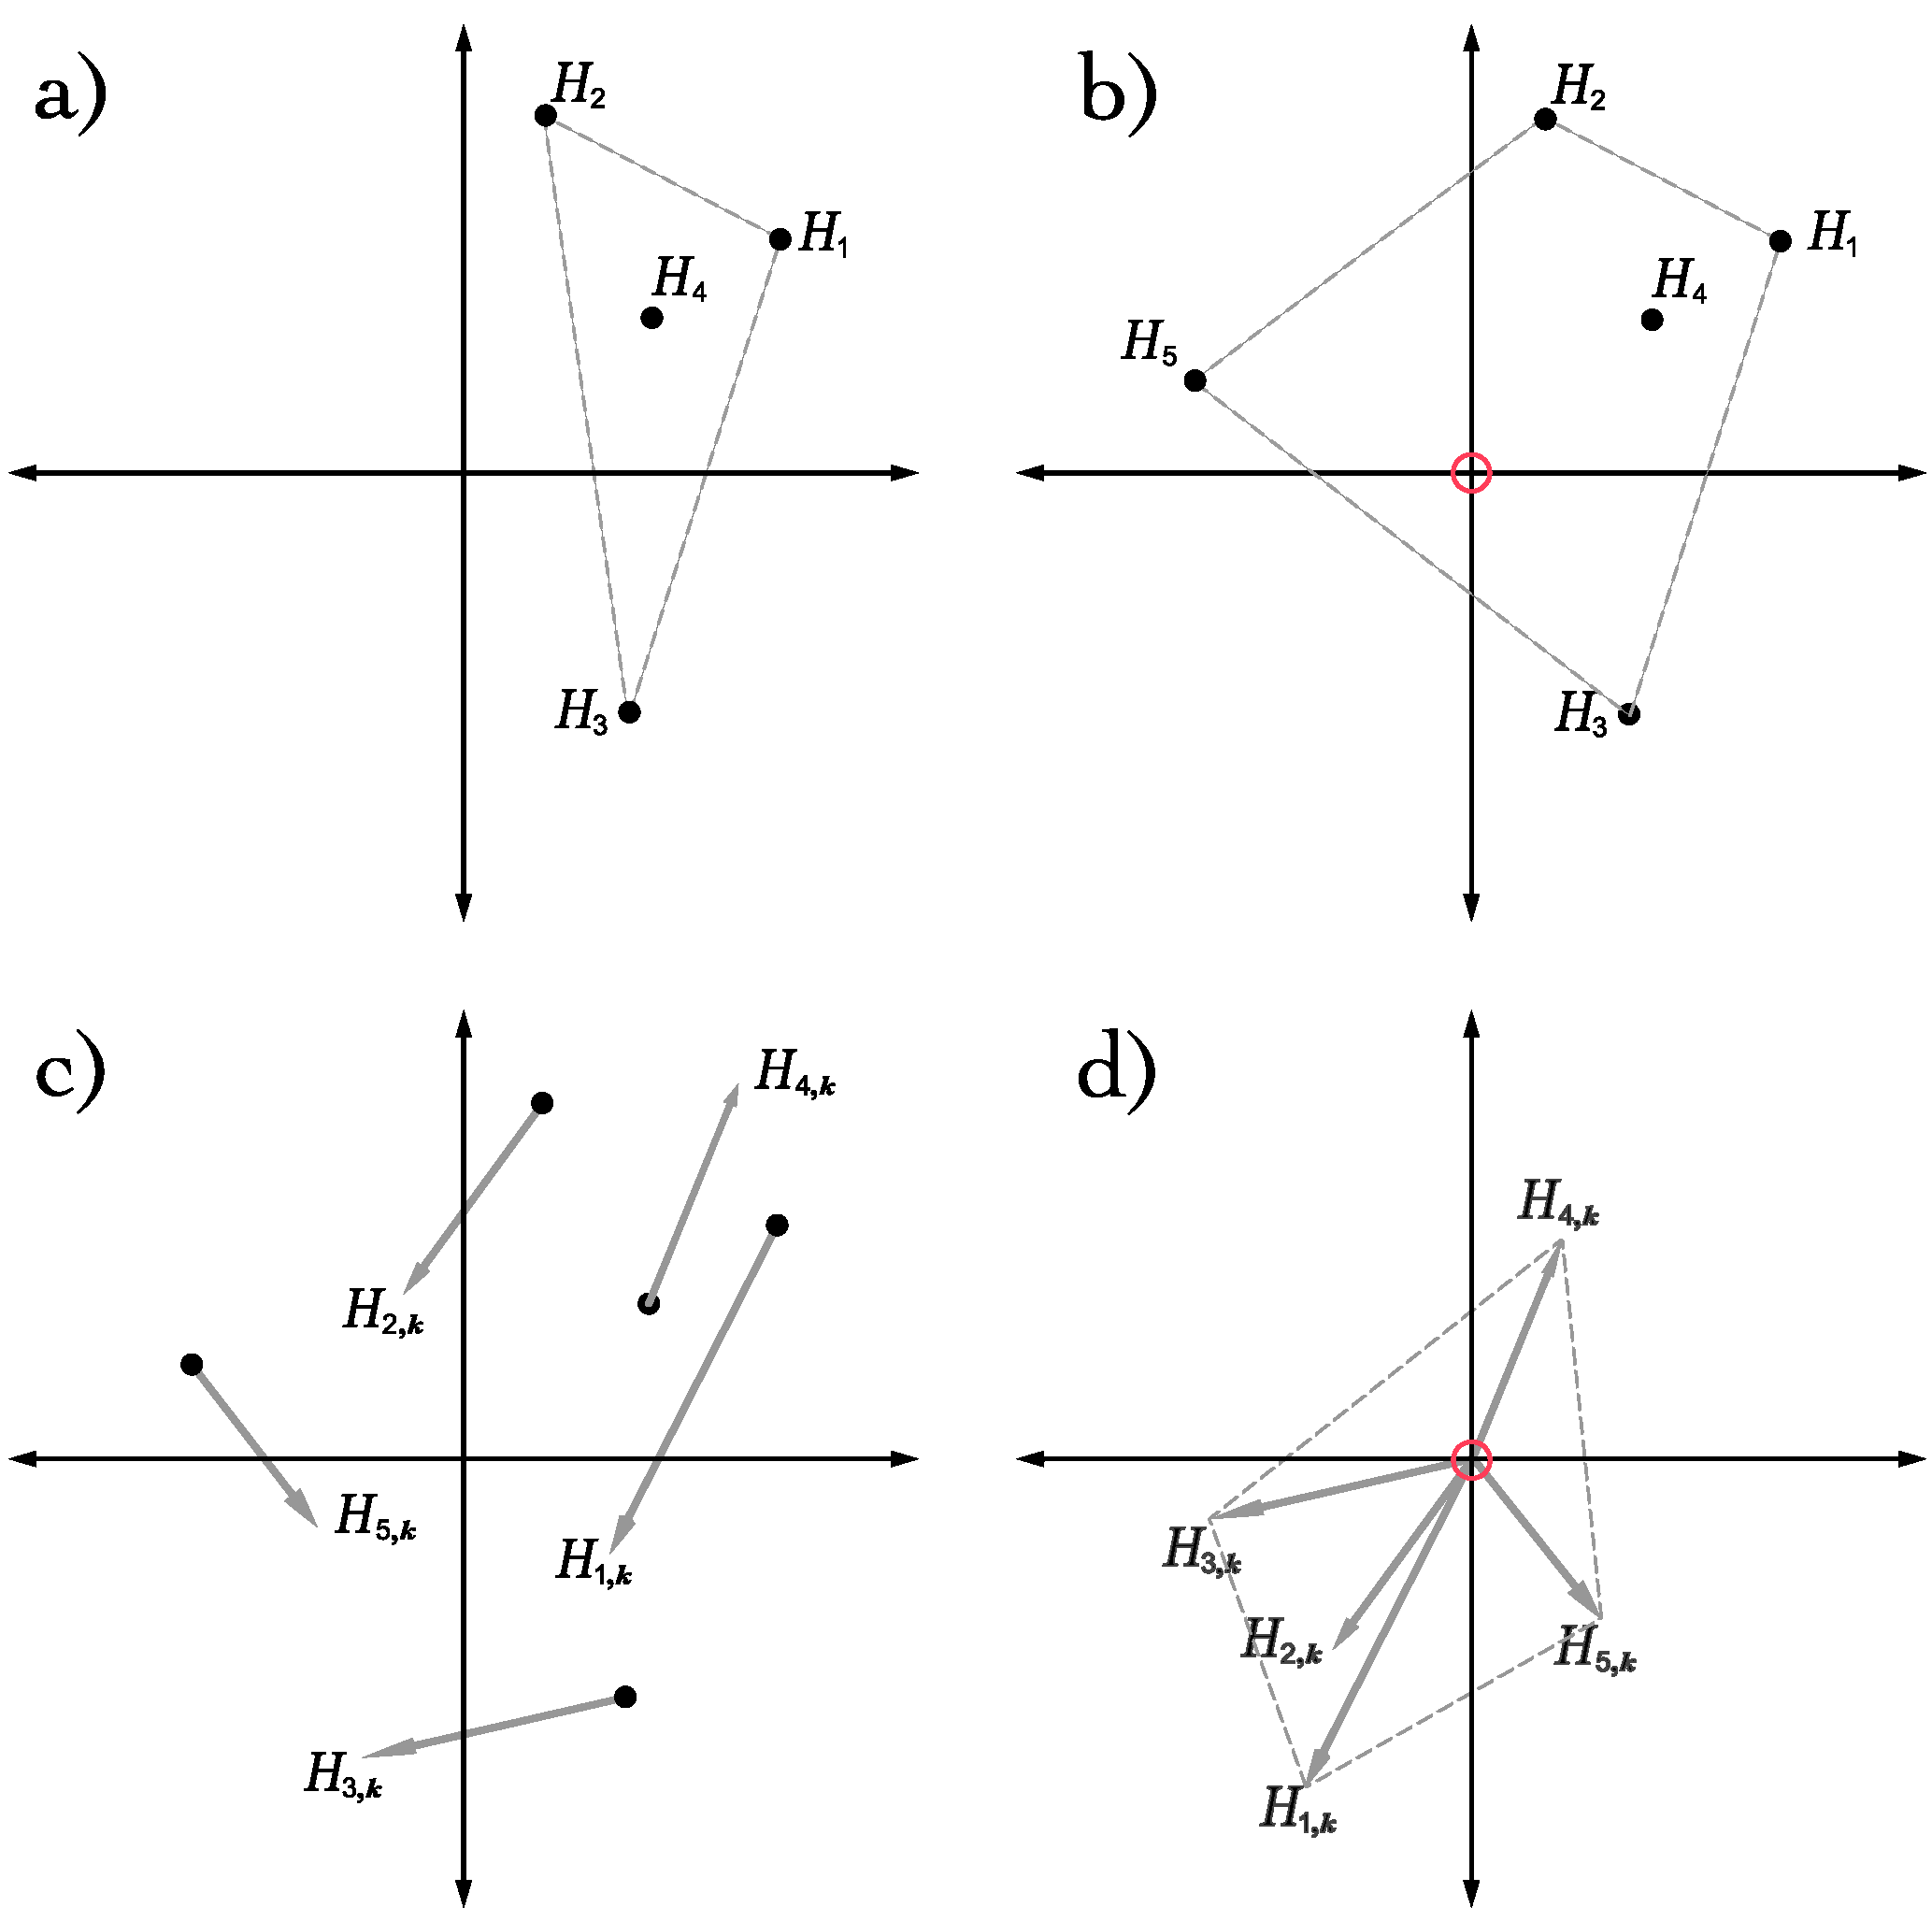
\includegraphics[width=\columnwidth]{vectorspace.pdf}
  \caption{A target unitary gate can be implemented a number of ways, each with a different effective Hamiltonian error. These error Hamiltonians lie in a vector space, which we illustrate as two-dimensional here. a) Four effective Hamiltonians. The origin is not contained in their convex hull, so there are no MQGs. b) After including an additional control solution, the convex hull grows to contain the origin, and so an MQG exists. c) The error Hamiltonians shown with their derivative with respect to a control parameter. As this parameter drifts, a MQG may drift, leading to a first-order error. d) The derivatives also lie in a vector space. If the origin lies in their convex hull, then it may be possible to construct a MQG.}
  \label{fig:vectorspace}
\end{figure}

While Campbell's approach can provide a guaranteed suppression of the error rate, it does not necessarily lead to a purely stochastic channel. Second- and higher-order terms in \eqref{eq:generators_and_effective_error} can easily contribute to lingering coherent errors that impact the efficient simulability of the channel. In order to definitively eliminate these coherent errors, we seek weights, $w_i$, that annihilate the off-diagonal entries of the unital submatrix of the effective error map, resulting in an effective error:
% \begin{equation}
% 	\mathcal{E}_{eff} = 
% 	\left(\begin{array}{@{}ccccc@{}}
% 		\cdot & \cdot & \cdot & \cdot \\ 
%   		\cline{1-1}\cline{3-4}
%     	\multicolumn{1}{|c}{0} & \multicolumn{1}{|c}{\cdot} & \multicolumn{1}{|c}{0} & \multicolumn{1}{c|}{0} \\
%     	\cline{2-2}\cline{3-3}		
% 		\multicolumn{1}{|c}{0} & 0 & \multicolumn{1}{|c}{\cdot} & \multicolumn{1}{|c|}{0}\\
% 		\cline{3-3}\cline{4-4}	
% 		\multicolumn{1}{|c}{0} & 0 & 0 & \multicolumn{1}{|c}{\cdot}\\
% 		\cline{1-3}
% 	\end{array} 	
% 	\right).
% \end{equation}

\begin{equation}
	\mathcal{E}_{\rm{eff}} = 
	\left(\begin{array}{@{}ccccc@{}}
		1 & 0 & 0 & 0 \\ 
    	0 &  p_x & 0 & 0 \\
		0 & 0 &  p_y & 0\\
		0 & 0 & 0 &  p_z\\
	\end{array} 	
	\right).
\end{equation}
The resulting mixed quantum gate is then guaranteed to have a Pauli stochastic error channel, and significantly increasing its simulability. We can formulate this problem analogously to the generator approach. The off-diagonal elements of the error map form a vector space, so we need only check that the origin is in the convex hull of the vectors of off-diagonal elements for each of the component operations, $\mathcal{E}_i$. 

In the remainder of this paper, we will formalize this process, presenting explicit convex optimizations to both generate a family of unitary controls and construct the optimal weighting vector. We will discuss how one might include additional desiderata, including a reduced sensitivity to environmental fluctuation as well as limiting the number of native unitaries that participate in the mixed gate. 

% \subsection{A simple example}
% \label{sec:simple_example}
% \noindent As a simple example of a mixed quantum gate, consider a single-qubit and two distinct implementations of a dynamically decoupled identity gate. Suppose that some control parameter, $\eta$, is prone to drift, causing each of these implementations to suffer a distinct, spurious phase error. These errors are equivalent to a small rotations about the $\sigma_z$ axis with angles $\theta = \{-\eta, 2\eta\}$. 
% % The resulting diamond distance errors and average gate fidelities of these four implementations are summarized in the following table:
% % \begin{center}
% % \begin{tabular}{|c|c|c|}
% % 	\hline
% % 	Rotation & Average gate  & Diamond  \\
% % 	angle &  infidelity & distance \\
% % 	$\theta$ & $\epsilon_{\mathcal{F}}$ & $\epsilon_{\diamond}$ \\
% % 	\hline\hline
% % 	${+2\eta}$ 	& $4\eta^2$  & $2\eta$\\
% % 	${+\eta}$ 	& $\;\eta^2$ & $\eta$ \\
% % 	${-\eta}$ 	& $\;\eta^2$ & $\eta$ \\
% % 	${-2\eta}$ 	& $4\eta^2$  & $2\eta$ \\
% % 	\hline
% % \end{tabular}
% % \end{center}
% % In such a scenario, if the ultimate goal is to produce a channel whose effect can be Monte Carlo simulated, then a useful approach would be to construct a channel whose errors are Pauli stochastic. Such a channel could be constructed, for instance, by drawing from this collection uniformly at random. More generally, given a collection of control, such a channel could be produced by minimizing the off-diagonal elements of $R$ in Equation \ref{eq:process_matrix}. 
% The error operators are then all of the form:
% \begin{equation}
% \mathcal{E}(\theta) = \exp(\theta \mathcal{L}_z) =
% 	\left(\begin{array}{ccccc}
% 		1 & 0 & 0 & 0 \\ 
% 		0 & \cos\theta & \sin\theta  & 0  \\
% 		0 & -\sin\theta & \cos\theta & 0  \\
% 		0 & 0 & 0 & 1
% 	\end{array} 	
% 	\right) 
% \end{equation}
% Where the z-axis generator, $\mathcal{L}_z$ is:
% \begin{equation}
% 	\mathcal{L}_z =
% 	\left(\begin{array}{ccccc}
% 		0 & 0 & 0 & 0 \\ 
% 		0 & 0 & -1  & 0  \\
% 		0 & 1 & 0 & 0  \\
% 		0 & 0 & 0 & 0
% 	\end{array} 	
% 	\right).
% \end{equation}
% The diamond distance associated with such an error is $\epsilon_\diamond(\mathcal{E}(\theta)) \simeq \theta$, while the fidelity is $\epsilon_\mathcal{F}(\error(\theta)) \simeq \theta^2$. Because 0 lies in the covex hull of the Following the Campbell procedure, we would assign weights $w = $





% If we were construct two channels, one with error $\error(\eta)$ and one with error $\error(-\eta)$, then we could construct a new channel with error $\error_{\rm eff} = \frac{1}{2}\left(\error(\eta) + \error(\eta)\right)$. The effective channel then has a matrix representation:
% \begin{equation}
% 	\error(\eta) =
% 	\left(\begin{array}{ccccc}
% 		1 & 0 & 0 & 0 \\ 
% 		0 & \cos\eta & 0  & 0  \\
% 		0 & 0 & \cos\eta & 0  \\
% 		0 & 0 & 0 & 1
% 	\end{array} 	
% 	\right) \simeq \mathcal{I} - 
% 	\left(\begin{array}{ccccc}
% 		0 & 0 & 0 & 0 \\ 
% 		0 & \eta^2/2 & 0  & 0  \\
% 		0 & 0 & \eta^2/2 & 0  \\
% 		0 & 0 & 0 & 0
% 	\end{array} 	
% 	\right)
% \end{equation}
% And with same average process fidelity, $\eta^2$, but now a suppressed diamond norm $\eta^2$. Now write this in terms of the error generators $\error(\eta) = \exp(\eta G)$ where
% \begin{equation}
% 	G =
% 	\left(\begin{array}{ccccc}
% 		0 & 0 & 0 & 0 \\ 
% 		0 & 0 & -1  & 0  \\
% 		0 & 1 & 0 & 0  \\
% 		0 & 0 & 0 & 0
% 	\end{array} 	
% 	\right)
% \end{equation}

% The effective generator vanishes at first order.




% In general, if we have a collection of single qubit controls $\{U_i\}$ generated by $\{H_i\}$, the channel that results from drawing from the controls probabilistically has elements given by:
% \begin{align}
% 	\mathcal{M}_{jk} 
% 		=& \sum_i p_i \tr{(\sigma_j^{\dagger}U\sigma_kU^{\dagger})} \\
% 		=& \sum_i p_i \tr{(\sigma_j^{\dagger} \exp(i \frac{\theta_i}{2} H_i)\sigma_k		\exp(-i \frac{\theta_i}{2} H_i)}) \\
% 		=& \tr (\sum_i p_i (\sigma_j^{\dagger}\sigma_k\cos\theta_i^2 + \sigma_j^{\dagger}H_i\sigma_k H_i\sin\theta_i^2 \\ 
% 		&+ i\sigma_j^{\dagger}H_i\sigma_k\sin\theta_i\cos\theta_i - i\sigma_j^{\dagger}\sigma_kH_i\sin\theta_i\cos\theta_i))
% \end{align}
% The first term corresponds to the identity, and $\sin\theta_i^2$ is always positive, so we cannot hope to eliminate the second term, but $\sin\theta_i\cos\theta_i$ may be positive or negative, and so there is hope that we could possibly combine various implementations to eliminate this term. The result would be a purely stochastic channel. 



% The problem of minimizing the last term:
% \begin{equation}
% \sum_i\sin\theta_i\cos\theta_i(\sigma_j^{\dagger}H_i\sigma_k - \sigma_j^{\dagger}\sigma_kH_i)
% \end{equation}
%  can equivalently be cast as trying to construct a family of vectors whose convex hull contains the origin. This can be seen in Figure \ref{fig:vectorspace} a) and b).



% ==============================================================================
% Section: Constructing Useful mixed quantum gates
% ==============================================================================
\section{Constructing mixed quantum gates}
\label{sec:mixed_unitary_processes}
\noindent In this section, we present a methodology for producing useful mixed quantum channels, formalizing the intuitive approach discussed above. As mentioned, our method requires two steps. The first is a control synthesis step, in which we construct an ensemble of gate implementations. Campbell and Hastings draw their ensembles from various different gate compilations, but for this work we use quantum optimal control theory to produce these ensembles. By running simple gradient descent algorithms, such as GRAPE \cite{Khaneja2005}, with different random initial seeds, one can quickly construct large ensembles of approximate quantum gates. We discuss this approach in some detail in Sec.~\ref{sec:numerical_results}. We note that advanced quantum control protocols may provide a more principled approach to control synthesis. DMORPH \cite{dominy2008exploring}, for example, provides a means of exploring continuous families of controls on fidelity level sets, thereby enabling further optimizations  fst secondary criteria, such as robustness or duration.  

The remainder of this section will focus on the second step of constructing the optimal weight vector to reduce the coherence of the effective error channel. We will begin by discussing two classes of optimization targets, i) cancelation of the first-order generator, and ii) elimination of the off-diagonal elements of the error channel. We then discuss a set of additions to the numerical optimization that can improve the performance by i) incorporating robustness to drift,  ii) targeting low-error-rate solutions, and iii) reducing the number of native unitaries that contribute to the effective channel. 

% In the examples that were discussed, all objective functions were linear, and reduced to finding a collection of controls whose convex hull contained the origin in some high-dimensional vector space. In those cases, the vectors might represent a collection of error generators or the off-diagonal elements of a collection of error maps. As we'll see in Section \ref{sub:adding_robustness}, we can also consider the derivatives of the error generators to minimize the sensitivity of the controls to drift. In this way, we see that by considering the appropriate collection of vectors, we can optimize our MQG for different purposes, and which routine we choose will depend on the quantities we are trying to minimize.

% ==============================================================================
% Section: Generators
% ==============================================================================
\subsection{Optimization Targets}
\subsubsection{First-order generators} % (fold)
\label{sub:first_order_generators}

Dnorm min:
\begin{equation}\label{eq:ddmin}
  \begin{split}
    &\underset{\omega_i\geq0, |\omega|_1=1}{\textbf{minimize}: } \hspace{.5cm} \epsilon_\diamond\left(\sum_i\mathsf{E}_i \omega_i\right)
  \end{split}
\end{equation}



One reason to construct an MQG is to improve the worst-case performance of a quantum gate. The worst-case performance is bounded by the diamond distance to the target, which would constitute a natural optimization target.  The diamond distance, however, is a non-linear function that in general requires a convex optimization to compute\cite{watrous2018theory}. This can dramatically slow down iterative optimizers, and so minimizing the diamond distance is a computationally expensive optimization target. However, if the errors are small enough, we can consider a linearized problem, minimizing the diamond distance to first-order in the effective error generator. As discussed in \cite{Campbell2017}, a sufficient condition to minimize the diamond distance of an MQG with error generators $\{\mathcal{L}_i\}$ to first order is:
\begin{equation}\label{eq:campbell-condition}
\sum \omega_i \mathcal{L}_i = 0
\end{equation}
In \cite{Campbell2017} Campbell presents an algorithm that, given an oracle that produces approximate unitary operations, will generate controls and weightings to find an MQG with this property. Alternatively, one might consider the following problem: \textit{Given a fixed collection of controls, how can I produce a weighting with minimal diamond norm?} Such a situation might arise if there is a natural family of controls that implement a desired gate, or if, as we consider later (Section \ref{sec:numerical_results}), we are given a collection of precomputed gate implementations. Given such an MQC we can consider the $n^2\times m$ matrix whose columns are the vectorized error generators:
\begin{equation}\label{eq:vectorized_generators}
	\bold{L} = \left(\begin{array}{cccc}
		\mathcal{L}_{1_{1,1}} & \mathcal{L}_{2_{1,1}} & \ldots   \\ 
		\vdots\ & \ddots &    \\
		\mathcal{L}_{1_{n,n}} &  &  \mathcal{L}_{m_{n,n}} \\ 
	\end{array} 	
	\right)
\end{equation}
To satisfy (\ref{eq:campbell-condition}), we can write the sum as a matrix product and solve the following optimization problem, which will be zero if and only if the sum is zero:

\begin{equation}\label{eq:minimization}
  \begin{split}
    &\underset{\omega_i\geq0, |\omega|_1=1}{\textbf{minimize}: } ||\bold{L}\omega||_2\\
  \end{split}
\end{equation}
where $||\cdot||_2$ is the $\ell_2$ norm.


As denoted, this optimization needs to be constrained so that $\omega$ is a proper probability distribution. Nevertheless, this forms a convex optimization problem, and such linearly constrained minimization problems with quadratic cost functions have been proven to be efficiently solvable by, e.g. the ellipsoid method \cite{wright1999numerical, khachiyan}. More importantly, there are many existing convex solver software packages that solve these problems efficiently in practice.

%In both cases it is clear that we should select the gates with smaller error, i.e. $\{U_{\epsilon}, U_{-\epsilon}\}$, rather than those with larger error, to minimize the multiplicative coefficient on the error. Despite this, literature commonly assumes that all controls are less than some threshold value, below which differences in performance don't matter. \cite{Campbell2017} In realistic scenarios, some controls will have better performance than others, and it is important to select from those controls when able to. We will discuss numerical approaches to solving this Section \ref{sec:norm}.

%Another interesting property of the MQG given in Equation \ref{eq:balanced} is that it maintains its first-order insensitivity even in the presence of drift. In particular, if the control amplitudes that implement these gates drift, they will drift in equal and opposite ways. Thus, the resulting depolarizing channel (see Figure \ref{fig:simple_example}) will have a time-dependent strength, but it will remain first-order insensitivity to the static detuning $\epsilon$. In Section \ref{sec:robustly_mixed} we will provide a method for producing controls that exhibit this robustness to drift to arbitrary order. Given these considerations from this simple example, we will now consider a numerical strategy for generating MQGs.


% subsection first_order_generators (end)

% ==============================================================================
% Section: Off-diagonals
% ==============================================================================

\subsubsection{Approximate Pauli Channel} % (fold)
\label{sub:off_diagonals}
There are other properties of a channel that one might consider optimizing. For instance, if an MQG has an error channel that is well-approximated by a Pauli-Stochastic channel, then it may be amenable to classical simulation. We can modify our optimization problem accordingly. By vectorizing the $R$ submatrices in (\ref{eq:process_matrix}), and considering the matrix of off-diagonal terms, we can again consider the minimization problem in (\ref{eq:minimization}), where we replace $\bold{L}$ with $\bold{R}$:

\begin{equation}\label{eq:vectorized_off_diagonal}
	\bold{R} = \left(\begin{array}{cccc}
		R_{1_{2,1}} & R_{2_{2,1}} & \ldots   \\ 
		\vdots\ & \ddots &    \\
		R_{1_{n-1,n-1}} &  &  R_{m_{n-1,n-1}} \\ 
	\end{array} 	
	\right)
\end{equation}

In this case, if (\ref{eq:minimization}) is satisfied, the resulting error channel will be \textit{exactly} a Pauli Channel. If this is achievable, then the circuit can be more efficiently simulated by Monte Carlo methods. Better yet, if the circuit consists of only Clifford gates, stabilizer methods can be used in conjunction with the Monte Carlo methods to give sub-exponential simulation times.\cite{quant-ph/9807006} Other authors have considered the problem of finding the closest Pauli or Clifford Channel to a given process \cite{Magesan2013, Puzzuoli2014} but, unlike our routine, this does not produce a channel that is decomposable into a given family of controls.

% subsection off_diagonals (end)

% ==============================================================================
% Section: Robustness
% ==============================================================================
\subsection{Additional Constraints}
\subsubsection{Adding robustness} % (fold)
\label{sub:adding_robustness}
While mixed quantum channels offer significant improvements to gate performance, they fail to take into account the reality that most control electronics experience drift over time scales relevant to QIP performance. Because of this drift, the quality of the MQG will degrade. Thus, we would like to design MQGs that are robust to this drift. To enforce robustness, we can consider the generators in (\ref{eq:campbell-condition}) to be functions of a control vector $\vec{\delta}$, and if the fluctuations are small enough, it is convenient to write the gate as a Taylor expansion in this small parameter:
\begin{equation}\label{eq:taylor}
\begin{gathered}
\tilde{\mathcal{G}_i}(d\vec{\delta}) = \exp(-i(\mathcal{L}_i(\vec{0}) + \frac{\partial}{\partial\delta_j}\mathcal{L}_i(\vec{0})d\delta_j\\ +  \frac{1}{2}\frac{\partial^2}{\partial\delta_j\partial\delta_k} \mathcal{L}_i(\vec{0})d\delta_j d\delta_k + \ldots))\mathcal{G}
\end{gathered}
\end{equation}

Now, instead of requiring that only the error generators average to zero, we can additionally impose a similar condition on the higher-order derivatives with respect to parameters that may drift. Specifically, we are interested in the $n^{th}$ order derivatives:
\kcy{Should the figures change from H to something else?}
\amp{Right. It seems to me they should be written as something like $D^1_{i,k}$. Then in the equation below I can use the comma notation, but for the $i^{th}$ derivative it's going to be some gross multi-index... I think your point is that the comma is standard notation (although I've never used it before.)}
\begin{equation}
\label{eq:derivative}
D^n_{i, (j_1, \ldots, j_n)} = \frac{1}{n!}\frac{\partial^{n}}{\partial\delta_{j_1}\ldots\partial\delta_{j_n}}\mathcal{L}_i(\vec{\delta})|_{\vec{\delta}=\vec{0}}
\end{equation}
If the dimension of $\vec{\delta}$ is $d$, the indices $j_1, \ldots, j_n$ take on values in $1, \ldots, d$ and this matrix has $d^n$ entries. 
We say that an MQG is robust to order $\ell$ (an $\ell$MQG) if for all $1 \leq k \leq \ell$:
\begin{equation}\label{eq:MQG}
\begin{gathered}
\sum_i\omega_i(\sum_{n=0}^k D^n_i)^n = 0\\
\end{gathered}
\end{equation}
In particular, we see that a 0MQG satisfies (\ref{eq:campbell-condition}). More generally, these conditions imply that an $\ell$MQG is insensitive to $\ell^{th}$ order in drift in $\vec{\delta}$. 
By Taylor expanding (\ref{eq:taylor}) in $d\vec{\delta}$, one can see that the the first $\ell$ derivatives of an $\ell$MQG will be zero. Furthermore if we can find controls such that $||D_i^n||\leq\alpha$, (\ref{eq:MQG}) is a pproximately satisfied in the sense that:
\begin{equation}\label{eq:MQG-relaxed}
\begin{gathered}
||\sum\omega_iD^n_i||+ \mathcal{O}(\alpha^2) = 0\\
\end{gathered}
\end{equation}
where $||\cdot||$ is the Frobenius norm. This condition guarantees, as before, that errors will be suppressed to second order in $\alpha$, but now for all derivatives up to order $\ell$. %A proof is included in the appendix that generalizes the Hastings-Campbell Mixing Lemma in \cite{Campbell2017}. Namely, Campbell showed that if $0\in $ Conv$[\{G_i(\vec{\delta})\}]$, where Conv is the convex hull of its arguments, then an $\vec{\omega}$ exists that quadratically decreases the diamond norm. We prove that $0\in $ Conv$[\{D_j^n(\vec{\delta})\}]$ implies there is an $\vec{\omega}$ exists that quadratically decreases the $\ell^{th}$-order sensitivity of the diamond norm of an $\ell$MQG.
As discussed in \cite{Campbell2017}, the geometric picture for 0MQGs is to consider the error generators as vectors, and to ensure zero is contained in their convex hull. Figure \ref{fig:vectorspace} generalizes this picture to 1MQGs and gives intuition for the conditions required to produce them. To generate $\ell$MQGs, we first define the vectorized derivative matrix ${\bold{D}^{\ell}}$ in a similar way to (\ref{eq:vectorized_generators}):
\begin{equation}
{\bold{D}^{\ell}} =  \left(\begin{array}{cccc}
		D^\ell_{1_{1,1}} & D^\ell_{2_{1,1}} & \ldots   \\ 
		\vdots\ & \ddots &    \\
		D^\ell_{1_{n,n}} &  &  D^\ell_{m_{n,n}} \\ 
	\end{array} 	
	\right)
\end{equation}

Using this, we can then solve the following convex optimization problem, generalizing (\ref{eq:minimization}):

\begin{equation}\label{eq:robust_minimization}
  \begin{split}
    &\underset{\omega_i\geq0, |\omega|_1=1}{\textbf{minimize}: } ||{\bold{D}^{\ell}}\omega||_1\\
    &\textbf{subject to: } \forall n<\ell, ||\sum \omega_iD_i^n||=0\\
  \end{split}
\end{equation}
with $D_n^i$ defined in (\ref{eq:derivative}). 

\begin{figure}
  \centering
  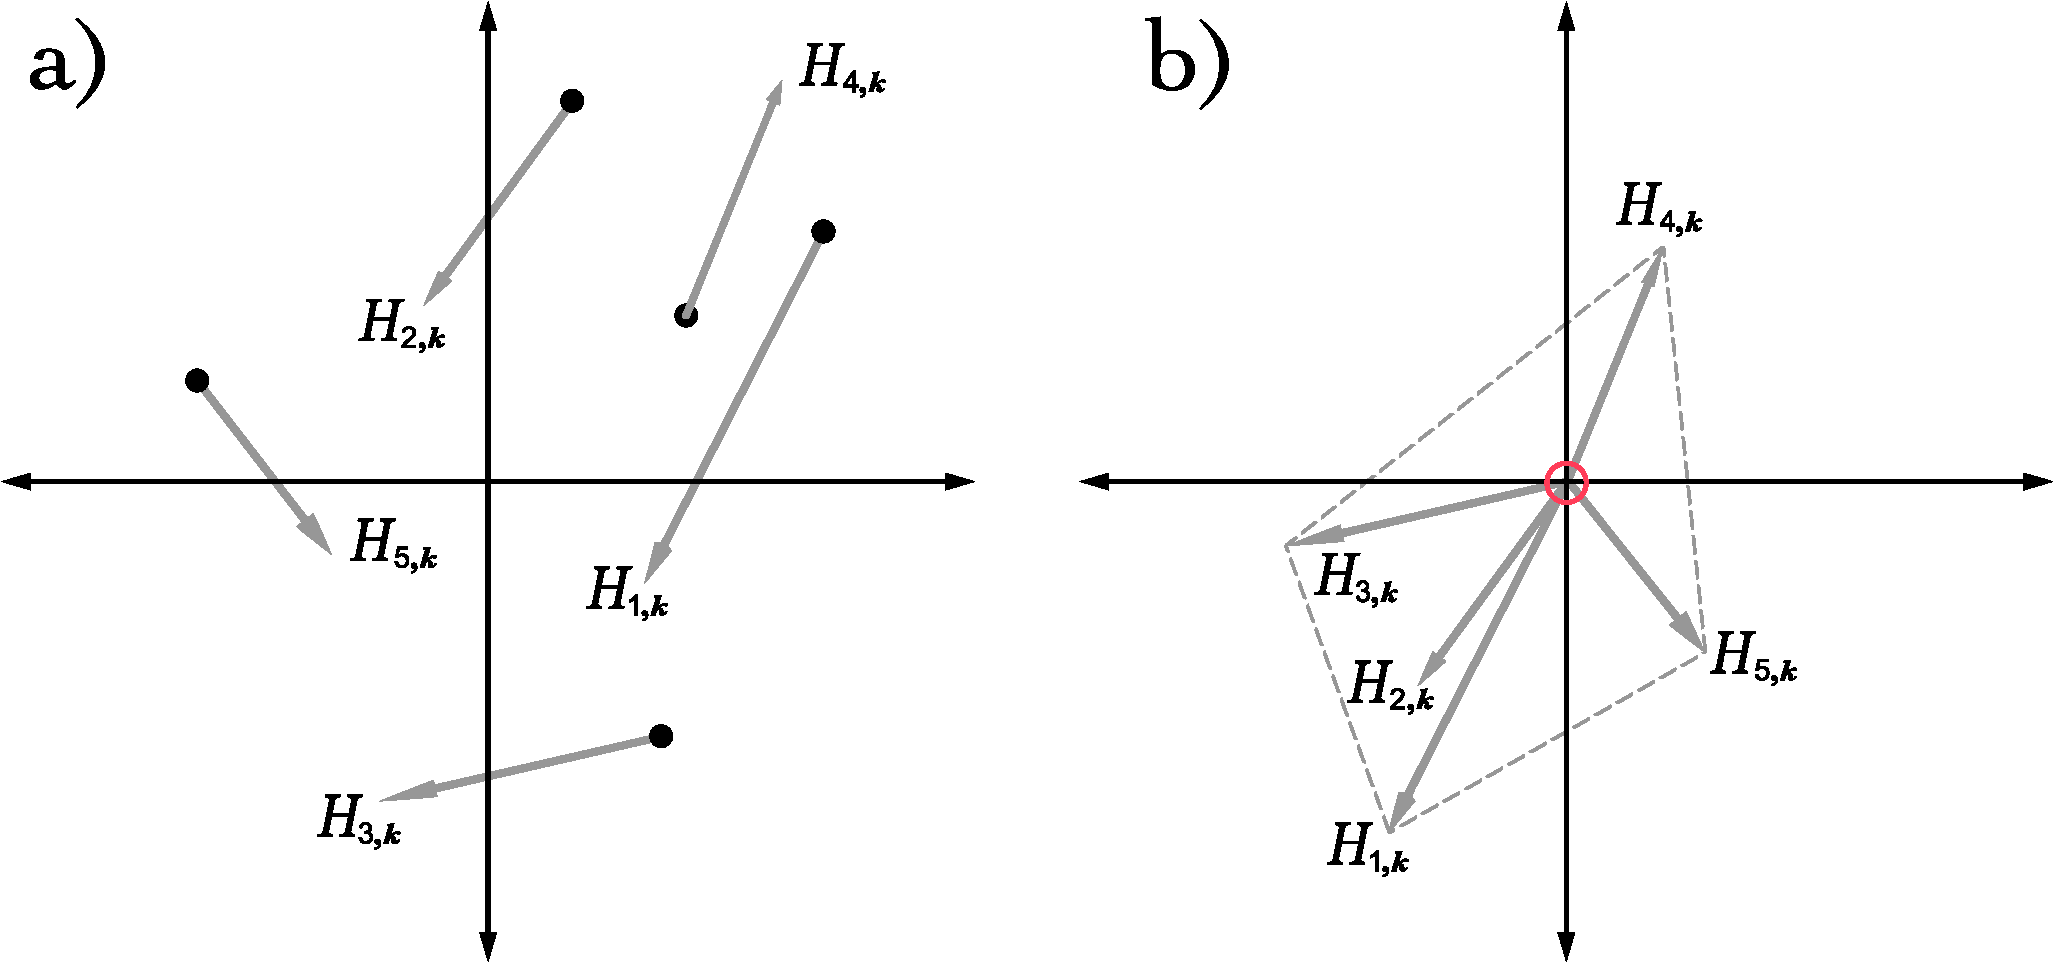
\includegraphics[width=\columnwidth]{vectorspace2.pdf}
  \caption{A target unitary gate can be implemented a number of ways, each with a different effective Hamiltonian error. a) The error Hamiltonians shown with their derivative with respect to a control parameter. As this parameter drifts, a MQG may drift, leading to a first-order error. b) The derivatives also lie in a vector space. If the origin lies in their convex hull $\mathsf{Conv}(\{H_k \otimes H_{k,1} \oplus H_{k,2} \oplus \cdots\}_k)$\amp{I'm not sure what you mean by the $_k$ subscript, nor why the tensor product is there. Also I think your indices are backwards?} then it may be possible to construct a robust 1-MQG. \kcy{This should appear in the main text somewhere. When we add the derivatives we make our space larger, but we still want the origin to be in the higher-dimensional convex hull.}}
  \label{fig:vectorspace}
\end{figure}

% subsection adding_robustness (end)

% ==============================================================================
% Section: Norm regularization
% ==============================================================================

\subsubsection{Hamiltonian Norm Regularization}
\label{sec:norm}
While quadratic programs with equality constraints have analytic solutions, the program we are considering has both constraints on the norm of the weight vector, and inequality constraints. Additionally, casting this problem as a convex optimization problem allows us to add penalty terms to the cost function to promote different properties of the MQG. In particular, while (\ref{eq:robust_minimization}) is sufficient for suppressing the diamond norm to first order relative to the \textit{worst} controls in the collection, it does not preferentially select the controls with the least error. As an example, any MQG that mixes equally over equal and opposite errors will satisfy (\ref{eq:robust_minimization}), but the magnitude of the error of the resulting channel will depend on the magnitude of the original coherent errors. To encourage the inclusion of controls with smaller error, we may impose a penalty proportional to the norm of the included Hamiltonians. In our case, we choose to penalize for the $\ell_2$ ($||\cdot||_2$) norm:

\newcommand{\bunderbrace}[2]{%
  \begin{array}[t]{@{}c@{}}
  #1\\
  \parbox{\widthof{#1}}{$\scriptscriptstyle#2$}
  \end{array}
}

\begin{equation}\label{eq:minimization_l2}
\begin{split}
& \ \bunderbrace{\textbf{minimize}: }{\omega_i\geq0, |\omega|_1=1} ||{\bold{D}^{\ell}}\omega||_1+ \eta\sum\omega_i||D^0_i||_2\\
&\ \ \textbf{subject to: } \forall n<\ell, ||\sum \omega_iD_i^n||=0\\
\end{split}
\end{equation}
with $\eta \geq 0$. By increasing $\eta$, we can encourage the optimizer to include better controls while minimizing the diamond norm. The value of $\eta$ that is best for any particular problem instance will depend on the values in $\bold{D}^\ell$.

%Naively generating the 1Q 0MQG in the previous section results in nontrivial support on all the members of the control family. However, as we will see in the next section, we can rewrite the minimization to impose a sparsity constraint, and the resulting 0MQG uses just five of the controls. 
% ==============================================================================
% Section: Sparsity
% ==============================================================================

\subsubsection{Sparsity Constraints}
\label{sec:sparsity}
As a practical consideration, we would also like to regularize our objective function to promote sparse weightings. Control electronics often have a limited amount of waveform memory, and thus it is important that MQGs only require a small number of controls. As an example, consider Figure \ref{fig:vectorspace}. In b), it is clear that $H_4$ is unnecessary to contain the origin in the convex hull of the error generators. Thus we would prefer that a $0$MQG exclude $H_4$. However, if we additionally want our controls to form a 1MQG, we see from d) that we need $H_4$ in our control set, in which case we would like our algorithm to exclude $H_1$, since its derivative is contained in the convex hull of the other controls' derivatives. 

In many machine learning contexts, lasso regularization \cite{tibshirani1996regression} can be used to enforce sparsity in solutions, however this is insufficient for our purposes, as we already constrain $\omega$ to be a valid probability distribution. Lasso regularization works by penalizing solutions with large $\ell_1$ norm, however if $\omega$ represents probabilities, it will always have an $\ell_1$ norm of one. Conveniently, the problem of enforcing sparsity in such situations has been considered in \cite{NIPS2012_4504} and can be expressed via another convex program that extends (\ref{eq:robust_minimization}):

\begin{equation}\label{eq:minimization_regularization}
\begin{split}
&\underset{n\in[N]}{\textbf{minimize}}\\
&\ \ \bunderbrace{\textbf{minimize}: }{\omega_i\geq0, |\omega|_1=1,\\ t\geq0} ||{\bold{D}^{\ell}}\omega||_1 + t\\
&\ \ \textbf{subject to: } \omega_n > \frac{\lambda}{t}\\
&\ \ \phantom{\textbf{subject to: }} \forall n<\ell, ||\sum \omega_iD_i^n||=0
\end{split}
\end{equation} with $\lambda\geq0$. As with $\eta$ in the last subsection, the optimal value of $\lambda$ is problem specific, depending on $\bold{D}^\ell$ and how sparse the solution needs to be. In the following sections we discuss both experimental and numerical implementations of MQGs, leveraging these optimization techniques. 

\section{Results} % (fold)
\label{sec:results}

% ==============================================================================
% Section: Experimental Results
% ==============================================================================

\subsection{Experimental} % (fold)
\label{sub:experimental}
In modern quantum computing platforms, diagnosing and correcting coherent errors remains a challenge. Methodologies like RPE and DRAG are sufficient for routinely achieving high single qubit fidelities in superconducting qubit architectures, however as coherence times increase, the community will continue to be interested in removing coherent errors to achieve higher fidelities. As a proof of principle, we implemented an MQG with a superconducting transmon qubit on the Rigetti 19Q-Acorn chip, whose performance we describe below. While this device consisted of 20 qubits with fixed couplings, here we will give results for a single qubit MQG on qubit 8. For more details about this particular device, characterization can be found in \cite{1712.05771}.

To implement an MQG on this qubit, we first calibrated a 10-sample, 50ns Gaussian pulse by coherently amplifying and correcting over- and under-rotation errors through repeated application. After the gate was sufficiently calibrated, four intentionally miscalibrated Gaussian pulses were produced by scaling the amplitude of the calibrated $RX(\frac{\pi}{2})$ pulse by $106.4\%$,  $103.9\%$, $93.7\%$ and $91.2\%$.

As discussed in Section \ref{sub:off_diagonals}, we chose to minimize the off diagonal elements of the process matrix. To benchmark the quality of the MQG, we then performed six randomized benchmarking experiments\cite{Magesan2011}: one for each over-- and under--calibrated pulse, one for the calibrated pulse, and one for the mixed process. We used $1000$ shots per experiment and $10$ sequences per sequence length, for sequence lengths of $2, 4, 8, 16, 32$ and $64$. In each case, our Clifford operations were decomposed into RX($\frac{\pi}{2})$ and RY($\frac{\pi}{2})$. In our implementation, these gates are implemented using the same pulse envelope definitions and control electronics, phase shifted by $\frac{\pi}{2}$ radians, and are therefore subject to identical miscalibration errors. The results are shown in Figure \ref{fig:rb} for sequence lengths $L=64$. Fitting to the randomized benchmarking decay curves, we find one-qubit gate fidelities of $99.3\%$ for the calibrated pulse, $98.9\%$ for Pulse1, $99.1\%$ for Pulse2, $98.9\%$ for Pulse3, $98.5\%$ for Pulse4, and $99.2\%$ for the MQG, demonstrating that it performs almost as well as the calibrated pulse, and better than the constituent pulses. 
\begin{figure}[t]
  \centering
  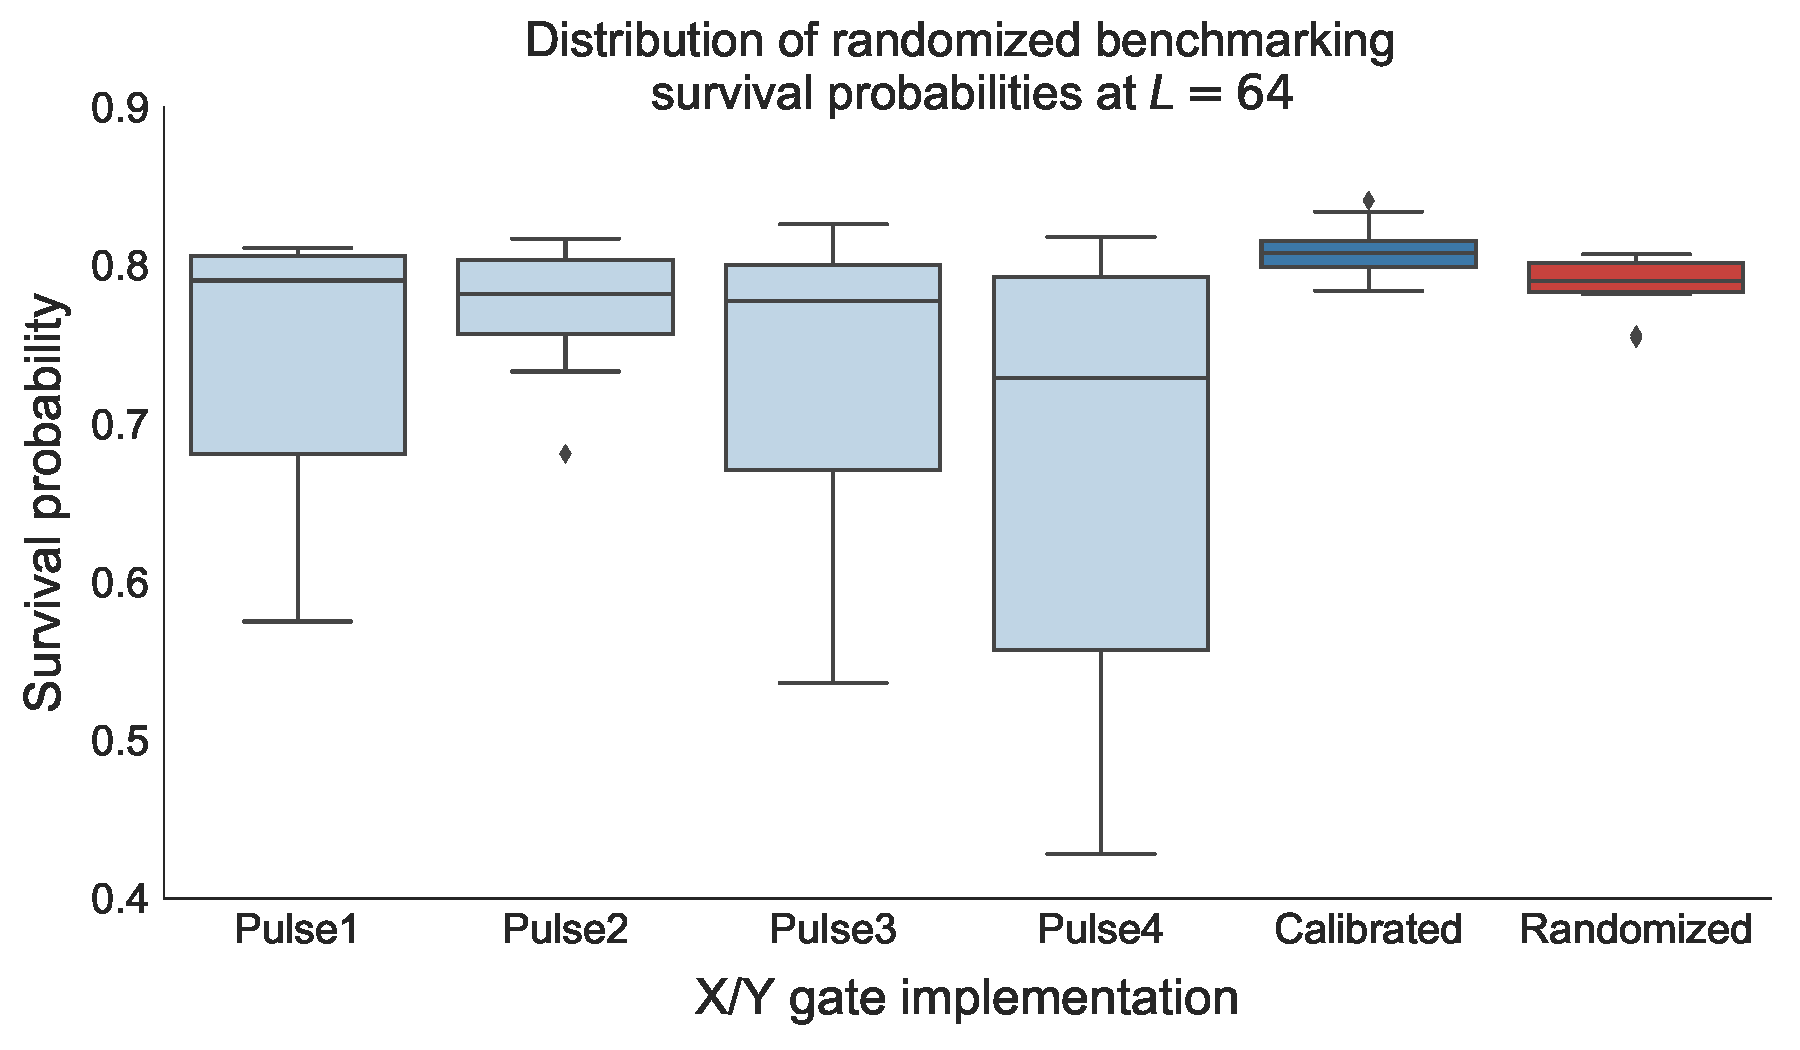
\includegraphics[width=\columnwidth]{rb_data.pdf}
  \caption{Randomized benchmarking experiments ran using different pulse definitions. The first four boxes result from using each of four different implementations of the ${\pi/2}$ rotations. The coherent noise present in these implementations leads to large variance of the survival probability over sequences. The fifth (dark blue) box illustrates the survival probability using a highly-tuned gate implementation. It displays improved average survival probability as well as reduced variance. The final box (dark red) illustrates the distribution over survival probabilities for a randomized MQG composed of Pulse1 through Pulse4. It performs comparably to the highly-calibrated implementation in both average survival probability and variance over random sequences. The reduced variance of the MQG is a tell-tale sign of reduced coherent error in the effective channel. }
  \label{fig:rb}
\end{figure}

More importantly, minimizing the off-diagonal elements of the process matrix, we expect to produce a process with suppressed coherent error. To see that this is the case, we can observe the drastic reduction in the variance at each point for the MQG relative to the miscalibrated pulses. A discussed in \cite{Ball2016}, for coherent error models, noise will manifest as gamma distributed points for each sequence length. On the other hand, incoherent noise, such as depolarizing noise, will result in Gaussian distributed fidelity estimates for each randomized benchmarking sequence length. We see that the coherently miscalibrated controls in our RB experiment have long tails, consistent with gamma distributed random variables, while the calibrated and randomized implementations both have much shorter tails, consistent with Gaussian distributed random variables. Thus our experiment demonstrates that the MQG has a significantly less-coherent error channel.
% subsection experimental (end)


% ==============================================================================
% Section: Numerical Results
% ==============================================================================
\subsection{Numerical Implementation}
\label{sec:numerical_results}
In the following numerical results, we use the methods in Section \ref{sec:mixed_unitary_processes} to build MQGs, and then analyze their performance for a range of Hamiltonian parameters. More specifically, we will construct a family of controls with some degree of inherent robustness to drift, and leverage the numerical techniques introduced to assign each control a probability. When drawn from with these probabilities, the controls will form an MQG with enhanced robustness to drift on the control parameters. We consider the following dimensionless model for a single tunable qubit: 
\begin{equation}\label{eq:1Qham}
  H(\delta, \epsilon, t) = \epsilon\sigma_z + (1 + \delta)(c_x(t)\sigma_x + c_y(t)\sigma_y)
\end{equation}
where $\epsilon$ corresponds to fluctuations in qubit frequency and $\delta$ corresponds to fluctuations in the control field.

To generate the initial controls, we use the GRAPE algorithm\cite{Khaneja2005} with N=25 steps and total evolution time of $\pi$ to generate 100 candidate controls. However, by imposing the sparisty constraint discussed in Section \ref{sec:sparsity}, we found MQGs consisting of just 10 controls. In our implementation of the GRAPE algorithm, we use the performance function presented in \cite{Khaneja2005}, and average over different values of $\delta$ and $\epsilon$ using Gaussian quadrature when computing the gradient, so that we find controls that are naturally robust. The standard deviations considered for all parameters in our numerical experiments were fixed to $\sigma=.001$. Finally, we assume that the errors on $\sigma_x$ and $\sigma_y$ are perfectly correlated, as in our experimental implementation.

Using controls generated in this way, the MQGs produced for $RX(\frac{\pi}{2})$ and $RY(\frac{\pi}{2})$ are qualitatively similar, with the results for $RX(\frac{\pi}{2})$ shown in Figure \ref{fig:YMQG}. By imposing the penalty from Section \ref{sec:norm}, we sought to ensure that the algorithm preferentially selected controls with smaller errors. Adding this constraint increased the performance of the 0MQG by nearly an order of magnitude at the origin, and produced a 1MQG whose performance is an order of magnitude better than the 0MQG away from the origin. Imposing this constraint allows us to trade off flatness for performance. This shows that through adding constraints to our optimization routine, we can make the MQG practically useful. 

\begin{figure}[h]
  \centering
  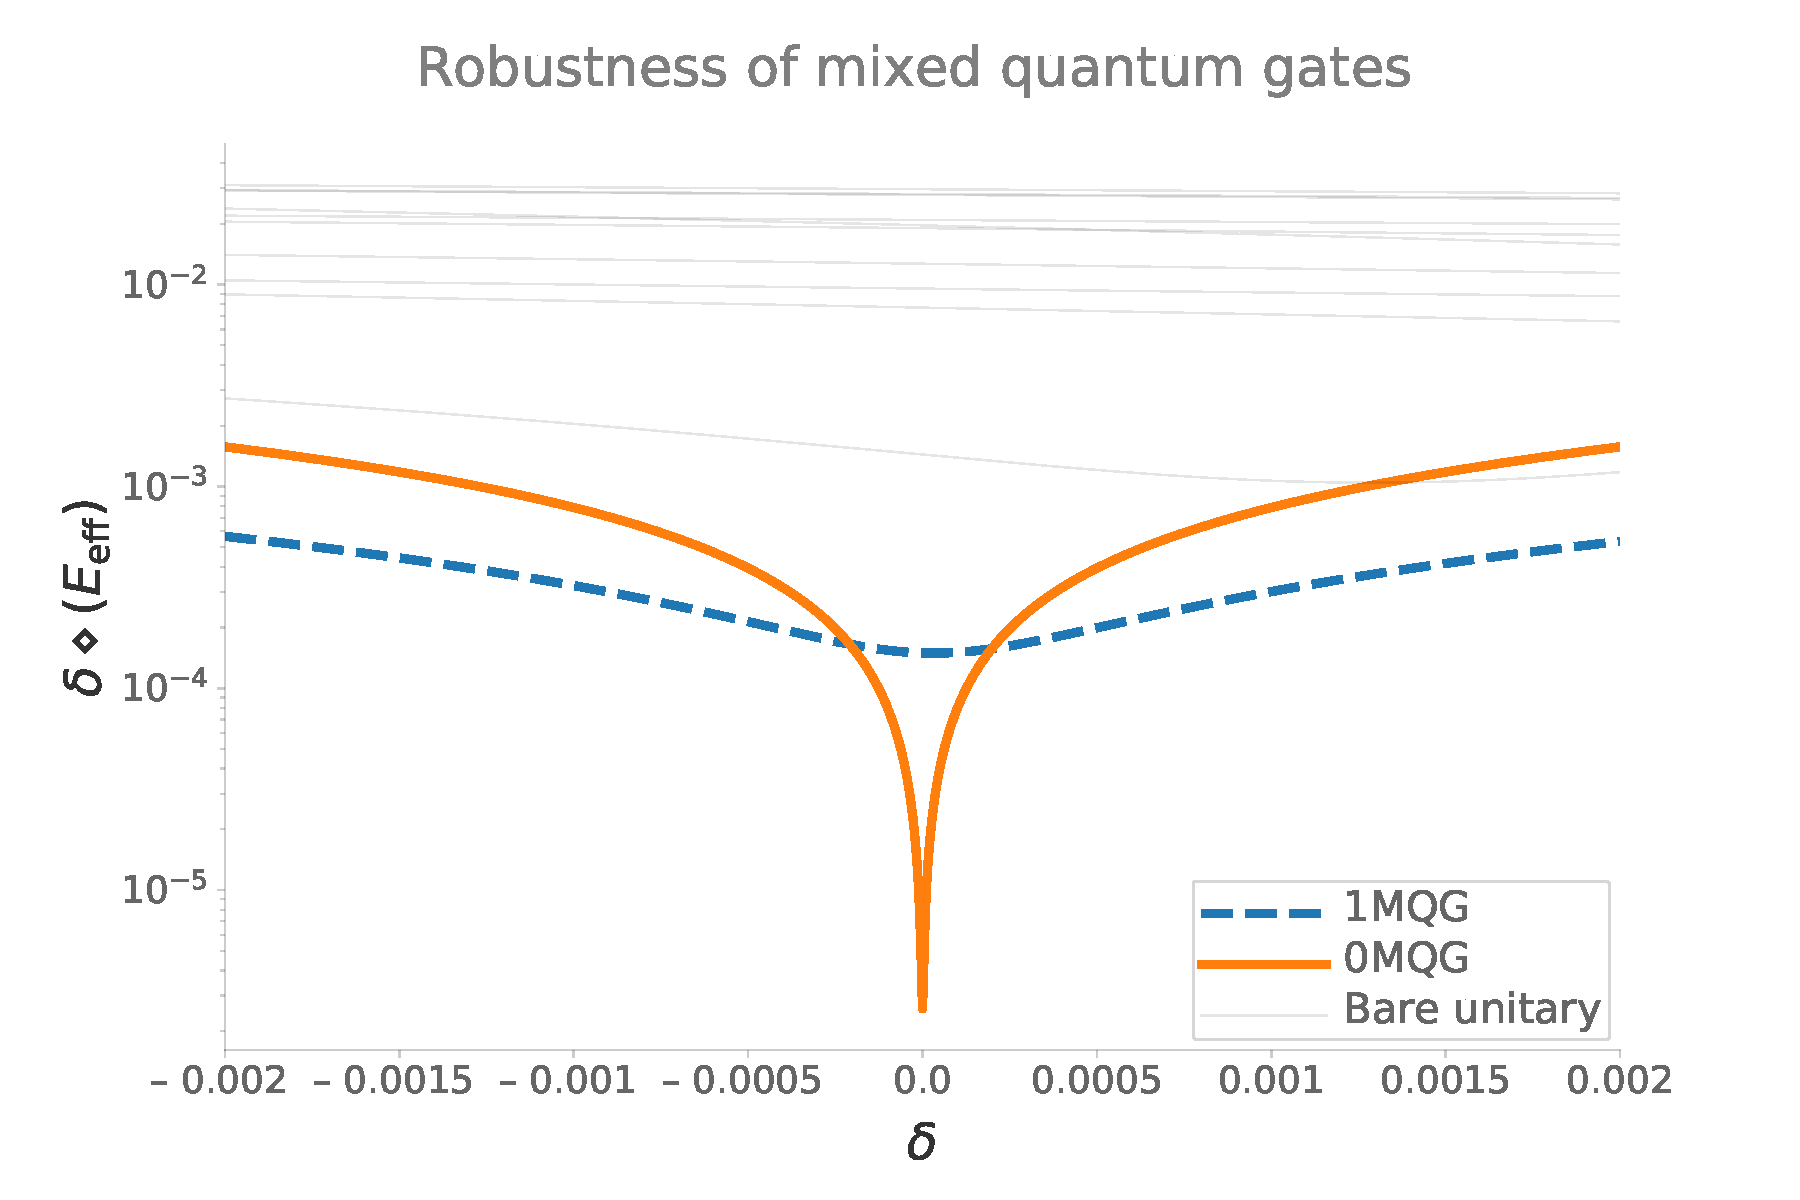
\includegraphics[width=\columnwidth]{figures/1q_robustness_delta.pdf}
  \caption{\amp{needs to be on previous page?}Numerical results comparing a 0MQG to a 1MQG for a single tunable qubit, for $RX(\frac{\pi}{2})$. The results are qualitatively similar to those for $RY(\frac{\pi}{2})$. In this case the 0MQG outperforms both the 1MQG by two orders of magnitude, and the constituent controls by three orders of magnitude at the origin. However, varying over $\delta$ we see that the 1MQG outperforms the 0MQG by up to an order of magnitude.}
  \label{fig:YMQG}
\end{figure}

In our two-qubit example we consider the following model for two tunable qubits coupled by a resonant exchange interaction, similar to that in \cite{McKay2016}:
\begin{equation} \label{eq:2Qham}
\begin{split}
H(\vec{\delta}, \vec{\epsilon}, t) = &\sum_{j=1}^2(\epsilon_j\sigma_z^j + (1 + \delta_j)(c_x^j(t)\sigma_x^j + c_y^j(t)\sigma_y^j)) \\
&+ \frac{1}{10}(XX + YY)
\end{split}
\end{equation}

\amp{This section is still tough to read, but I'm not sure of a better way to handle it. The constituent controls are clearly contrived, so I think it best to be explicit about how they were constructed.}In this example it was infeasible to use GRAPE to return non-trivial solutions. Instead we manually selected piecewise constant echoing sequences with 500 steps and total evolution time of $\frac{5\pi}{2}$. In particular, we considered $RX(\pi)$, $RX(-\pi)$, $RY(\pi)$ and $RY(-\pi)$ bang-bang sequences \cite{bangbang}, consisting of all combinations of simultaneous $\pi$ pulses activated at multiples of $8$ steps from the beginning of the controls, and the same multiple of $8$ steps prior to the end of the controls. To give the control family a variety of RF errors, we also added uniformly distributed amplitude errors to each $\pi$ pulse, between $-.25$\% and $.25$\%.

In this example, we find more modest improvements to performance, as shown in Figure \ref{fig:2MQG}. There are now four free parameters to optimize over, and the uncontrolled entangling interaction means that there is little room for variation in the controls. Nonetheless, using an MQG improves performance by half an order of magnitude at the origin relative to the constituent controls, and up to an order of magnitude away from the origin. For all values of the drifting parameters we see that the 1MQG performs as well or better than 0MQG.

\begin{figure}
  \centering
  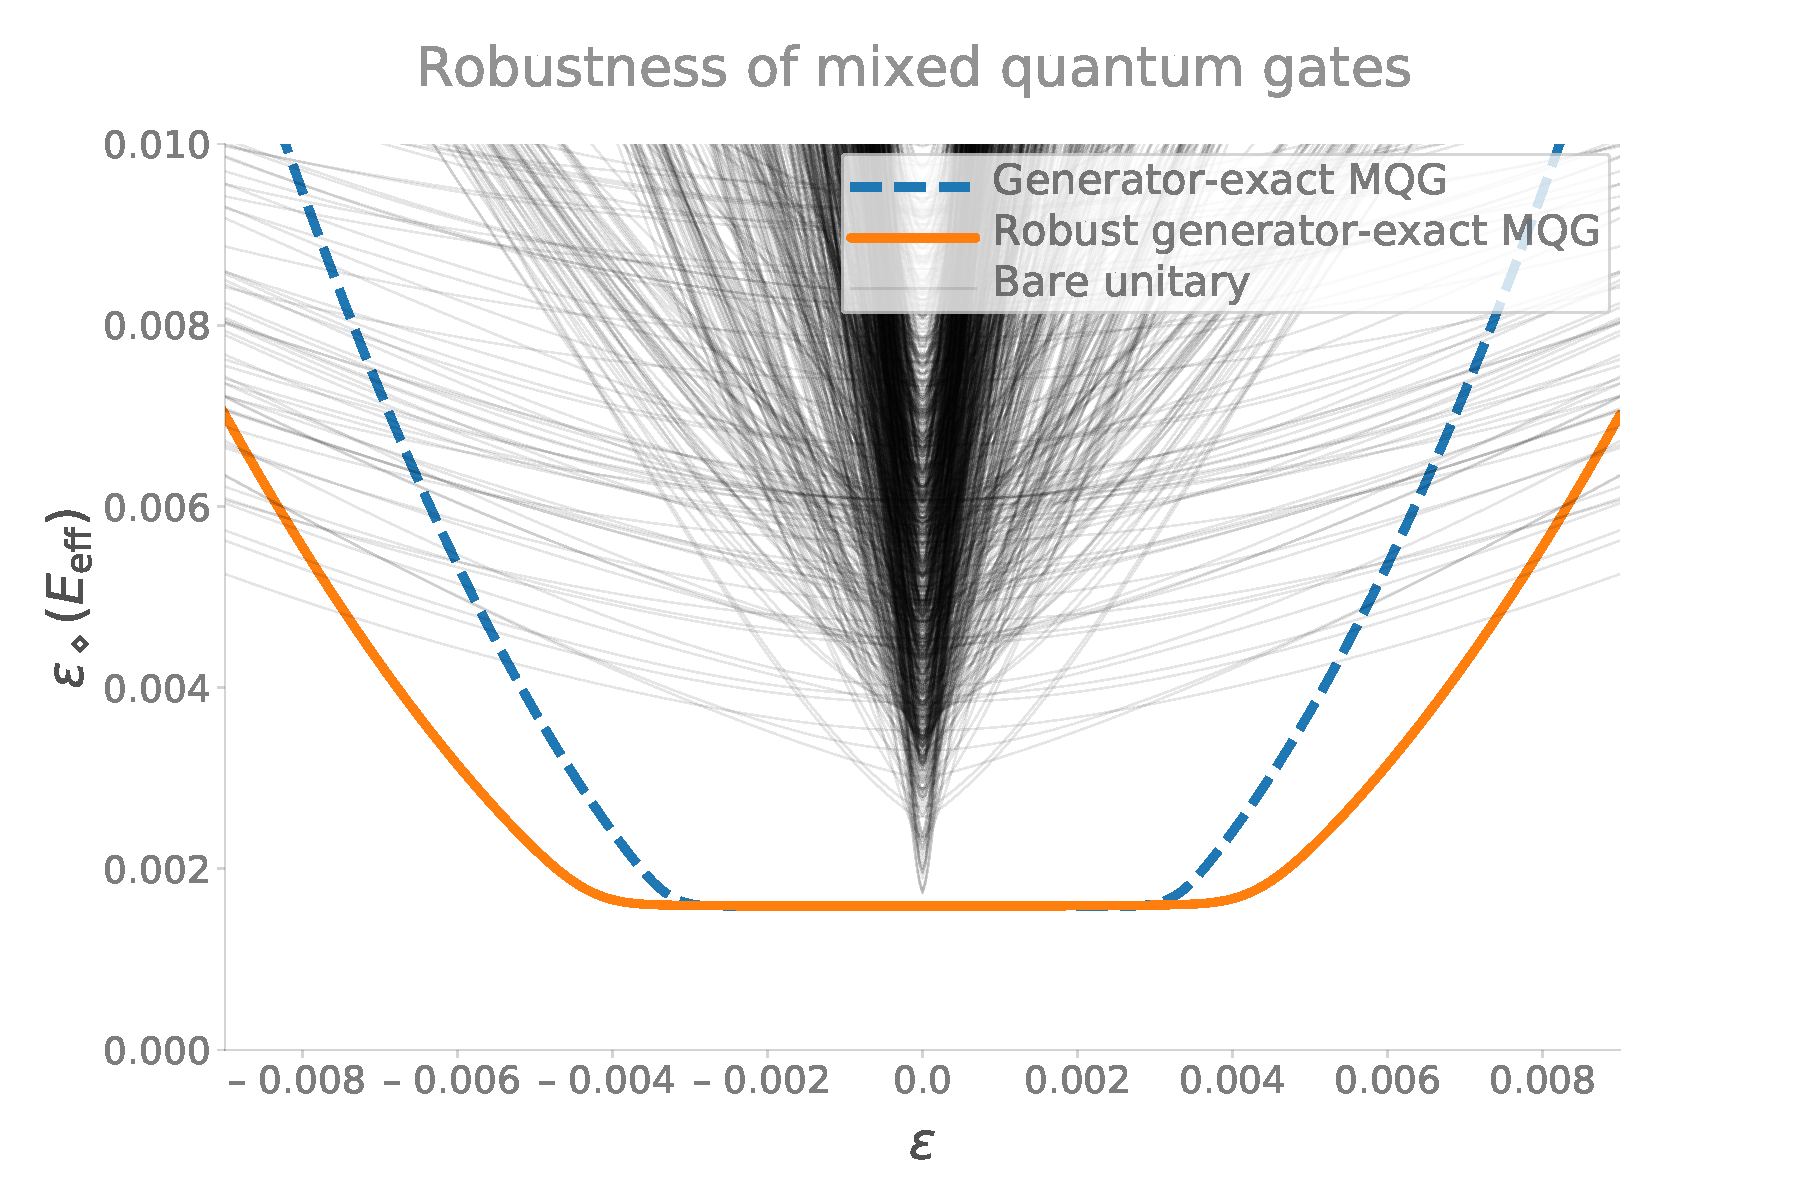
\includegraphics[width=\columnwidth]{figures/2q_robustness.pdf}
  \caption{\kcy{needs to be on previous page} Numerical results comparing a 0MQG to a 1MQG for a pair of tunable qubits, with a resonant exchange interaction. Shown with lower alpha values are example constituent controls. The 0MQG and 1MQG can be seen to outperform these controls by half of an order of magnitude at the origin. For all detuning values the 1MQG performs as well or better than the 0MQG. When there is $.2\%$ drift in the qubit frequency, the 1MQG outperforms members of the control families by almost an order of magnitude in diamond norm. Similarly, for $.2\%$ drift in the qubit control amplitude, we see that the 1MQG outperforms the the constituent controls by over half an order of magnitude.}
  \label{fig:2MQG}
\end{figure}






% ==============================================================================
% Section: Conclusion and Future Work
% ==============================================================================


\section{Conclusion and Future Work}
We have shown numerically that using MQGs can reduce coherent error by more than an order of magnitude in diamond norm, over a wide range of quasi-static values of noise. In addition, we have demonstrated that these approximate controls can be generated through optimal control (GRAPE), and that the minimization problem is tractable.

Randomized protocols have a long history of outperforming their deterministic counterparts. In \cite{Viola2005, Santos2006} the use of randomness is discussed in the context of dynamical decoupling. In particular, it is shown that both stochastic and hybrid approaches can result in better or more tractable coherent controls. Additionally Pauli Frame Randomization\cite{Wallman2016} has been shown \cite{1803.01818} to reduce coherent errors by introducing randomness in a pre-compilation step. The techniques discussed in this paper are different from both of these approaches in that they explicitly produce incoherent errors through mixing, and that the randomness is hardware efficient for any desired gate.

Future directions for this work include demonstrating the routine experimentally on a two-qubit gate, moving the random gate selection from a pre-compilation step to runtime logic onboard the control electronics, investigating other optimization routines such as CRAB \cite{Caneva2011} and GOAT\cite{Machnes2018}, and using more sophisticated benchmarking routines such as GST\cite{BlumeKohout2017} to quantitatively investigate the performance of our method.

Another interesting area of research would be using model-free approaches. The numerical work in the paper assumes access to a model of the system, however an experimentalist may not have a model readily available to describe the system, e.g. in the presence of unknown on-chip crosstalk, or an uncalibrated transfer function of the system. Even if a model is available, it might be computationally inconvenient to simulate, i.e. for more than a few qubits. In these situations, one approach would be to use \textit{in-situ} optimal control techniques \cite{Wu2018, Kelly2014, Ferrie2015} to generate candidate controls, and then use an optimizer like Nelder-Mead to perform the minimization. While performing a complete optimization in this way would require full process tomography, one could instead optimize via partial tomography. By selecting pre-- and post --rotations that correspond to measuring Pauli-moments of interest in the Hamiltonian, such as unwanted $Z\otimes Z$ crosstalk, one could perform optimization over fewer parameters.


% ==============================================================================
% Section: Acknowledgements
% ==============================================================================

\section{Acknowledgements}
\label{sec:acknowledgements}
This material was funded in part by the U.S. Department of Energy, Office of Science, Office of Advanced Scientific Computing Research Quantum Testbed Program. Sandia National Laboratories is a multimission laboratory managed and operated by National Technology and Engineering Solutions of Sandia, LLC, a wholly owned subsidiary of Honeywell International, Inc., for the U.S. Department of Energy's National Nuclear Security Administration under contract DE-NA0003525.
\bibliography{mixed_unitaries.bib}


\newpage
% \onecolumngrid
% ==============================================================================
% Section: Appendix
% ==============================================================================
\section{Appendix}
\label{sec:appendix}

% ==============================================================================
% Section: Diamond Distance Inequality
% ==============================================================================
\subsection{Diamond distance inequality}
\label{sub:diamond_distance_inequality}
Here we prove the claim of \eqref{eq:diamond_ineq} that:
\begin{equation}
	\epsilon_\diamond\!\left(\mathsf{E}_{\rm eff}\right) \le \sum w_i \, \epsilon_\diamond(\mathsf{E}_i).
\end{equation}
The effective error channel for a mixed quantum gate is $\mathsf{E}_{\rm{eff}} = \sum w_i\,\mathsf{E}_i$, where $\mathsf{E}_i$ are the error channels for the component gates. The diamond distance to the identity of the effective error channel is:
\begin{align}
	\epsilon_\diamond \left(\mathsf{E}_{\rm eff}\right)
		&= \frac{1}{2} \sup_\rho \vert \vert (\mathsf{I}_d\otimes \mathsf{I}_d)(\rho) 
										  - (\mathsf{E}_{\rm eff} \otimes \mathsf{I}_d)(\rho) \vert\vert_1\\
		% &= \frac{1}{2} \sup_\rho \vert \vert (\mathsf{I}_d\otimes \mathsf{I}_d)(\rho) 
										  % - (\sum_i w_i\,\mathsf{E}_i \otimes \mathsf{I}_d)(\rho) \vert\vert_1 \\
		&= \frac{1}{2} \sup_\rho \vert \vert \sum w_i\,((\mathsf{I}_d
										  - \mathsf{E}_i) \otimes \mathsf{I}_d)(\rho) \vert\vert_1
\end{align}
For qubits, the space of density matrices is compact, so the supremum is achievable. Call a state that achieves the supremum $\rho^*$. Then 
\begin{align}
	\epsilon_\diamond \left(\mathsf{E}_{\rm eff}\right)
		&= \frac{1}{2} \vert \vert \sum w_i\,((\mathsf{I}_d
										  - \mathsf{E}_i) \otimes \mathsf{I}_d)(\rho^*) \vert\vert_1 \\
		&= \frac{1}{2} \vert \vert \sum w_i\, \rho^*_i \vert\vert_1,
\end{align}
where we have defined $\rho^*_i = ((\mathsf{I}_d - \mathsf{E}_i) \otimes \mathsf{I}_d)(\rho^*)$. The nuclear norm above is equal to the sum of the singular values of $\sum w_i \rho_i$. Using the Ky Fan singular value inequality \cite{fan1951maximum} , we have 
\begin{align}
	\epsilon_\diamond \left(\mathsf{E}_{\rm eff}\right)
		&\le \frac{1}{2} \sum_i w_i \vert \vert \rho^*_i \vert\vert_1 \\
		&\le \sum_i w_i\, \epsilon_\diamond(\mathsf{E}_i)
\end{align}
The second inequality above follows because $\rho^*$ defines an explicit lower bound for the diamond distance for each of the component error maps. 

% % subsection diamond_distance_inequality

% \subsection{Robust Mixing Lemma}
% \label{sub:rml}
% We begin by generalizing Lemma 2 from \cite{Campbell2017}. If all of our error Hamiltonians $\{H_j\}$ have bounded error, that is:
% \begin{equation}
% ||H_j||\leq c
% \end{equation}
% Then we may consider the derivative of any mixture of unitaries as:
% %\begin{equation}
% %\deriv\sum_j \omega_je^{iH_j} = \deriv(\id + (\sum_ji%\omega_jH_j) + \sum \omega_j\sum_{n=2}^{\infty}%\frac{(iH_j)^n}{n!}))
% %\end{equation}
% \begin{equation}
% \deriv\sum_j \omega_je^{iH_j} = \sum_j\omega_ji\deriv (H_j)e^{iH_j}
% \end{equation}
% By assumption, the derivatives of the first order term sum to zero, and so we see by A3 in \cite{Campbell2017} that
% \begin{equation}
% ||\deriv\sum_j\omega_je^{iH_j}|| \leq \sum_j\omega_j||i\deriv (H_j)(iH_j + \sum_{n=2}^{\infty}\frac{(iH_j)^n}{n!})|| \leq \sum_j\omega_j(c^2 + \frac{c^2}{2}) \leq c^2 + \frac{c^3}{2}
% \end{equation}
% Where we have used the fact that $||AB|| \leq ||A||||B||$ with $||\cdot||$ being the $\infty$-norm.
% Additionally, 
% \begin{align}
% ||\deriv e^{iH_j}|| &= ||\deriv(iH_j)e^{iH_j}|| \\
% &\leq ||\deriv(iH_j)|| + ||\deriv(iH_j)H_j|| +  ||\deriv(iH_j)\sum^{\infty}_{n=2}\frac{1}{(n)!}(iH_j)^n|| \\
% &\leq ||\deriv(iH_j)|| + ||\deriv(iH_j)||\cdot||H_j|| +  ||\deriv(iH_j)||\cdot||\sum^{\infty}_{n=2}\frac{1}{(n)!}(iH_j)^n||\\
% &\leq c + c^2 + \frac{c^3}{2}
% \end{align}
% And so we see that Lemma 2 generalizes. We will use the above to upper bound the 1-norm (and hence diamond norm) in the following.

% Next we generalize the Mixing Lemma from \cite{Campbell2017}. We must assume that the 1-norm is uniformly differentiable. In that case, we see that:

% \begin{align}
% &= \deriv\sup|\mathcal{I}\otimes\mathcal{I}-\error(\vec{\delta})\otimes\mathcal{I}|_1 \\
% &= \sup\deriv|\mathcal{I}\otimes\mathcal{I}-\error(\vec{\delta})\otimes\mathcal{I}|_1 \\
% &\leq \sup|\deriv(\mathcal{I}\otimes\mathcal{I}-\error(\vec{\delta})\otimes\mathcal{I})|_1 \\
% \end{align}
% And so we see it is sufficient to upperbound:
% \begin{equation}
% |\deriv(\mathcal{I}\otimes\mathcal{I}-\error(\vec{\delta})\otimes\mathcal{I})|_1
% \end{equation}
% From Equation 18 in \cite{Campbell2017}:
% \begin{align}
% &(\mathcal{V}\circ\mathcal{E} - \id)(X) = \sum_j \omega_j(\tilde{\delta}_jX + X\tilde{\delta}_j^{\dagger} + \tilde{\delta}_jX\delta_j^{\dagger})\\
% &\deriv(\mathcal{V}\circ\mathcal{E} - \id)(X) = \sum_j \omega_j(\deriv\tilde{\delta}_jX + X\deriv\tilde{\delta}_j^{\dagger} + \deriv\tilde{\delta}_jX\delta_j^{\dagger} + \tilde{\delta}_jX\deriv\delta_j^{\dagger})\\
% \end{align}
% Thus, by H\"older's inequality we find:
% \begin{align}
% &||\deriv(\mathcal{V}\circ\mathcal{E} - \id)(X)||_1\leq||\sum_j \omega_j\deriv\tilde{\delta}_j|| + ||\sum_j\omega_j\deriv\tilde{\delta}_j^{\dagger}|| + \sum_j\omega_j|| \deriv\tilde{\delta}_j||\cdot||\delta_j^{\dagger}|| + \sum_j\omega_j||\tilde{\delta}_j||\cdot||\deriv\delta_j^{\dagger}||
% \end{align}
% By assumption, all of these terms are neglible, and therefore we find:
% \begin{align}
% ||\deriv(\mathcal{V}\circ\mathcal{E} - \id)(X)||_1\leq 2a^2 + 2b^2
% \end{align}
% And so we see that the mixing lemma extends to first order. In a similar way, it can be extended to arbitary order, and thus if we can find constructions that satisfy the generalized Lemma 2, we can use the Robust Mixing Lemma to conclude that there exists a weighting with linearly supressed diamond norm.


\end{document}
